\documentclass{protokol}
\usepackage{graphicx}
\usepackage{float}

\usepackage{tikz}
\usetikzlibrary{calc}
\usetikzlibrary{arrows}


%====== Units =====
\usepackage{amssymb}
\usepackage{siunitx}
\sisetup{inter-unit-product =\ensuremath{\cdot}}
\sisetup{group-digits = integer}
\sisetup{output-decimal-marker = {,}}
\sisetup{exponent-product = \ensuremath{\cdot}}
\sisetup{separate-uncertainty}
\sisetup{tight-spacing = false}
%\sisetup{scientific-notation = true}
%\sisetup{round-mode=places,round-precision=4}
%\sisetup{evaluate-expression}


%====== Grafy =====
\usepackage{pgfplots}
\pgfplotsset{width=0.8\linewidth, compat=1.17}
\def\plotcscale{0.8}
\usepackage{pgfplotstable}
\usepackage[figurename=Obr.]{caption} % figure caption rename

\usepackage[siunitx]{circuitikz} % obvody
% \ctikzset{bipoles/length=1cm}

%====== Rovnice align block ======
\usepackage{amsmath}
\setlength{\jot}{10pt} % rozestup mezi řádky

\graphicspath{ {./img/} }

%====== Code blocks ======
\usepackage{listings}

\usepackage[most]{tcolorbox}
\newtcbox{\inlinecode}{on line, boxsep=0pt, left=2pt, right=2pt, top=2pt, bottom=2pt, colframe=gray, boxrule=0.5pt, arc=1pt, auto outer arc, before upper={\vphantom{dlg}}, tcbox raise base} % vytvoření inline boxu pro kód

\lstdefinelanguage{Spice}{
    alsoletter={.},  % Přidává tečku jako součást slov
    morekeywords={.lib, .STEP, .param, .MEAS, FIND, WHEN, END, VALUE, R, C, L, K, .SUBCKT, .ENDS, .MODEL, .INCLUDE, .AC, .DC, .TRAN, .PRINT, .PLOT, .PROBE, .WIDTH, .OPTIONS, .NODESET, .IC},
    keywordstyle=\color{blue}\bfseries,
    sensitive=false, % klíčová slova nejsou citlivá na velikost písmen
    morecomment=[l]{;}, % komentáře začínají hvězdičkou
    morestring=[b]", % řetězce uzavřené do uvozovek
}

\lstset{
  language=Spice,
  basicstyle=\ttfamily\small,
  breaklines=true,
  numbers=left,
  numberstyle=\tiny\color{gray},
  frame=single,
  rulecolor=\color{black},
  title=\lstname,
  keywordstyle=\color{blue}\bfseries,
  commentstyle=\color{green},
  stringstyle=\color{red},
  showstringspaces=false
}

%====== Vyplňte údaje ======
\jmeno{Tomáš Vavrinec}
\kod{240893}
\rocnik{}
\obor{MET}
\skupina{}
\spolupracoval{--}

\merenodne{--}
\odevzdanodne{--}
\nazev{Extrakce parametrů tranzistorů MOSFET ze~SPICE~modelu}
\cislo{1} %měřené úlohy

\predmet{Návrh analogových integrovaných obvodů}
\ustav{Ústav mikroelektroniky}
\skola{FEKT VUT v~Brně}

\def\para{x+0}
\def\parb{\para-80}


%citace 
\usepackage[backend=biber, style=iso-numeric, sortlocale=cs_CZ, autolang=other, language=czech]{biblatex}
\addbibresource{bibliography.bib}
\DeclareFieldFormat{labelnumberwidth}{\mkbibbrackets{#1}}
% hyperlinky
\usepackage[colorlinks]{hyperref}

% odstavce
\usepackage{parskip}

% Bloky kódu
\usepackage{xcolor}

%New colors defined below
\definecolor{codegreen}{rgb}{0,0.6,0}
\definecolor{codegray}{rgb}{0.5,0.5,0.5}
\definecolor{codepurple}{rgb}{0.58,0,0.82}
\definecolor{backcolour}{rgb}{0.95,0.95,0.92}

\usepackage{listings}
\lstdefinestyle{mystyle}{
  backgroundcolor=\color{backcolour}, commentstyle=\color{codegreen},
  keywordstyle=\color{magenta},
  numberstyle=\tiny\color{codegray},
  stringstyle=\color{codepurple},
  basicstyle=\ttfamily\footnotesize,
  breakatwhitespace=false,         
  breaklines=true,                 
  captionpos=b,                    
  keepspaces=true,                 
  numbers=left,                    
  numbersep=5pt,                  
  showspaces=false,                
  showstringspaces=false,
  showtabs=false,                  
  tabsize=2
}
\lstset{
	inputencoding=utf8,
	extendedchars=true,
	literate={á}{{\'a}}1 {č}{{\v{c}}}1 {ď}{{\v{d}}}1 {é}{{\'e}}1 {ě}{{\v{e}}}1 
           {í}{{\'i}}1 {ň}{{\v{n}}}1 {ó}{{\'o}}1 {ř}{{\v{r}}}1 {š}{{\v{s}}}1 
           {ť}{{\v{t}}}1 {ú}{{\'u}}1 {ů}{{\r{u}}}1 {ý}{{\'y}}1 {ž}{{\v{z}}}1 
           {Á}{{\'A}}1 {Č}{{\v{C}}}1 {Ď}{{\v{D}}}1 {É}{{\'E}}1 {Ě}{{\v{E}}}1 
           {Í}{{\'I}}1 {Ň}{{\v{N}}}1 {Ó}{{\'O}}1 {Ř}{{\v{R}}}1 {Š}{{\v{S}}}1 
           {Ť}{{\v{T}}}1 {Ú}{{\'U}}1 {Ů}{{\r{U}}}1 {Ý}{{\'Y}}1 {Ž}{{\v{Z}}}1,
	style=mystyle
	}

% Číslování
\pagenumbering{arabic}



% =========================================
% =============== DOKUMENT ================
% =========================================
\begin{document}
	%====== Vygenerování tabulky ======
	\maketitle

\section*{ZADÁNÍ ÚLOHY}
  Detailní popis jednotlivých úloh s návodem najdete v NAO\_PC.pdf, který je dostupný v E-learningu.

\begin{itemize}
    \item {\bf Simulací získejte hodnoty prahového napětí \(U_{TH0}\) pro dvě různé řady rozměrů tranzistorů.}
    \begin{itemize}
        \item konstantní poměr \(W/L = 5, kdy \$L\$ = 0.18; 0.3; 0.5; 0.8; 1; 2; 3; 5; 10\),
        \item různé rozměry: \(W/L = 0.22/0.18; 1/0.5; 2/0.5; 2/1; 5/1; 5/2; 10/5; 10/10; 40/10\),
        \item výše uvedené dva body budou provedeny pro tranzistor NMOS i PMOS.
    \end{itemize}
    \item {\bf Závislost prahového napětí \(U_{TH}\) na \(U_{SB}/U_{BS}\) (bulk efekt) Simulací získejte hodnoty prahového napětí \(U_{TH}\) pro napětí \(U_{BS}\) (NMOS) resp. \(U_{SB}\) (PMOS) v rozsahu \(0 [V]\) až \(500 [mV]\) s krokem \(50 [mV]\).}
    \item {\bf Závislost parametru modulace délky kanálu (\(\lambda\)) na délce kanálu (L) Simulací získejte hodnoty parametru \(\lambda\) tranzistoru NMOS a PMOS pro L v rozmezí \(200 [nm]\) až \(10 [\mu m]\).}
\end{itemize}

\subsection*{Bonusové otázky (1 b.)}
\begin{itemize}
    \item Popište, jak byste simulací (mimo analýzu \inlinecode{.op}) zjistili transkonduktanci \(gm\).
          Nakreslete schéma, popište nastavení a odečet hodnot.
\end{itemize}

\setcounter{section}{0}

  \newpage
\section{Vypracování}
  \subsection{Transkonduktační parametr \(KP\)}  
  
\begin{figure}[H]
    \vspace{8mm}
    \begin{minipage}{0.5\textwidth}
        \begin{circuitikz}[scale=1, transform shape] 
            \draw
              % MOSFET transistor with labels for drain (D), gate (G), source (S), and bulk (B)
              (0,0) node[nmos, bulk] (mos) {}
              (mos.drain) node[left] {M1}
            
              % Gate voltage source VGS
              (mos.gate) to[short, -] ++(-2,0) to[voltage source, l^=$V_{GS}$] ++(0,-1.5) node[ground] {}
              
              % Drain voltage source VDS (vertical)
              (mos.drain) to[short, -] ++(0,1) -- ++(2,0) -- ++(0,-1) to[voltage source, l^=$V_{DS} $] ++(0,-2) -- (2,-1.5) node[ground] {}
              
              % Source connected to ground, aligned with VGS ground
              (mos.source) to[short, -] (0,-1.5) node[ground] {}
              
              % Bulk (body) connection to ground
              (mos.bulk) to[short, -] (0.5, 0) -- ++(0,-1) -- ++(-0.5,0)  node[circle,fill,inner sep=1pt] (myNode) {}
            ;
        \end{circuitikz}

        \vspace{5mm}
        \centering{(NMOS)}
    \end{minipage}
    \hfill
    \begin{minipage}{0.5\textwidth}
        \begin{circuitikz}[scale=1, transform shape] 
            \draw
              % MOSFET transistor with labels for drain (D), gate (G), source (S), and bulk (B)
              (0,0) node[pmos, bulk] (mos) {}
              (mos.drain) node[left] {M1}
                          
              % Gate voltage source VGS
              (mos.gate) to[short, -] (-2,0) to[voltage source, l^=$V_{GS}$] (-2,2) -- ++(2,0) node[circle,fill,inner sep=1pt] (myNode) {}
              
              % Drain voltage source VDS (vertical)
              (mos.source) to[short, -] (0,2) -- ++(2,0) -- ++(0,-1) to[voltage source, l^=$V_{DS} $] ++(0,-2) -- (2,-1.5) -- (0,-1.5)
              
              % Source connected to ground, aligned with VGS ground
              (mos.drain) to[short, ] (0,-1.5) node[circle,fill,inner sep=1pt] (myNode) {} (0,-1.5) node[ground] {}

              % Bulk (body) connection to ground
              (mos.bulk) to[short, -] (0.5, 0) -- ++(0,1) -- ++(-0.5,0)  node[circle,fill,inner sep=1pt] (myNode) {}

            %   (2,2)  to[short, *-o] ++(1,0) node[above, right]{$V_{CC}$}
            ;
        \end{circuitikz}

        \vspace{5mm} 
        \centering{(PMOS)}
    \end{minipage}
    \caption{\label{cod:cod_NP_WL_const} Zapojení pro určení \(U_{TH0}\) pro tranzistor NMOS a PMOS}
\end{figure}

\begin{figure}[h]
    \hspace{-20mm}
    \begin{minipage}{0.5\textwidth}
        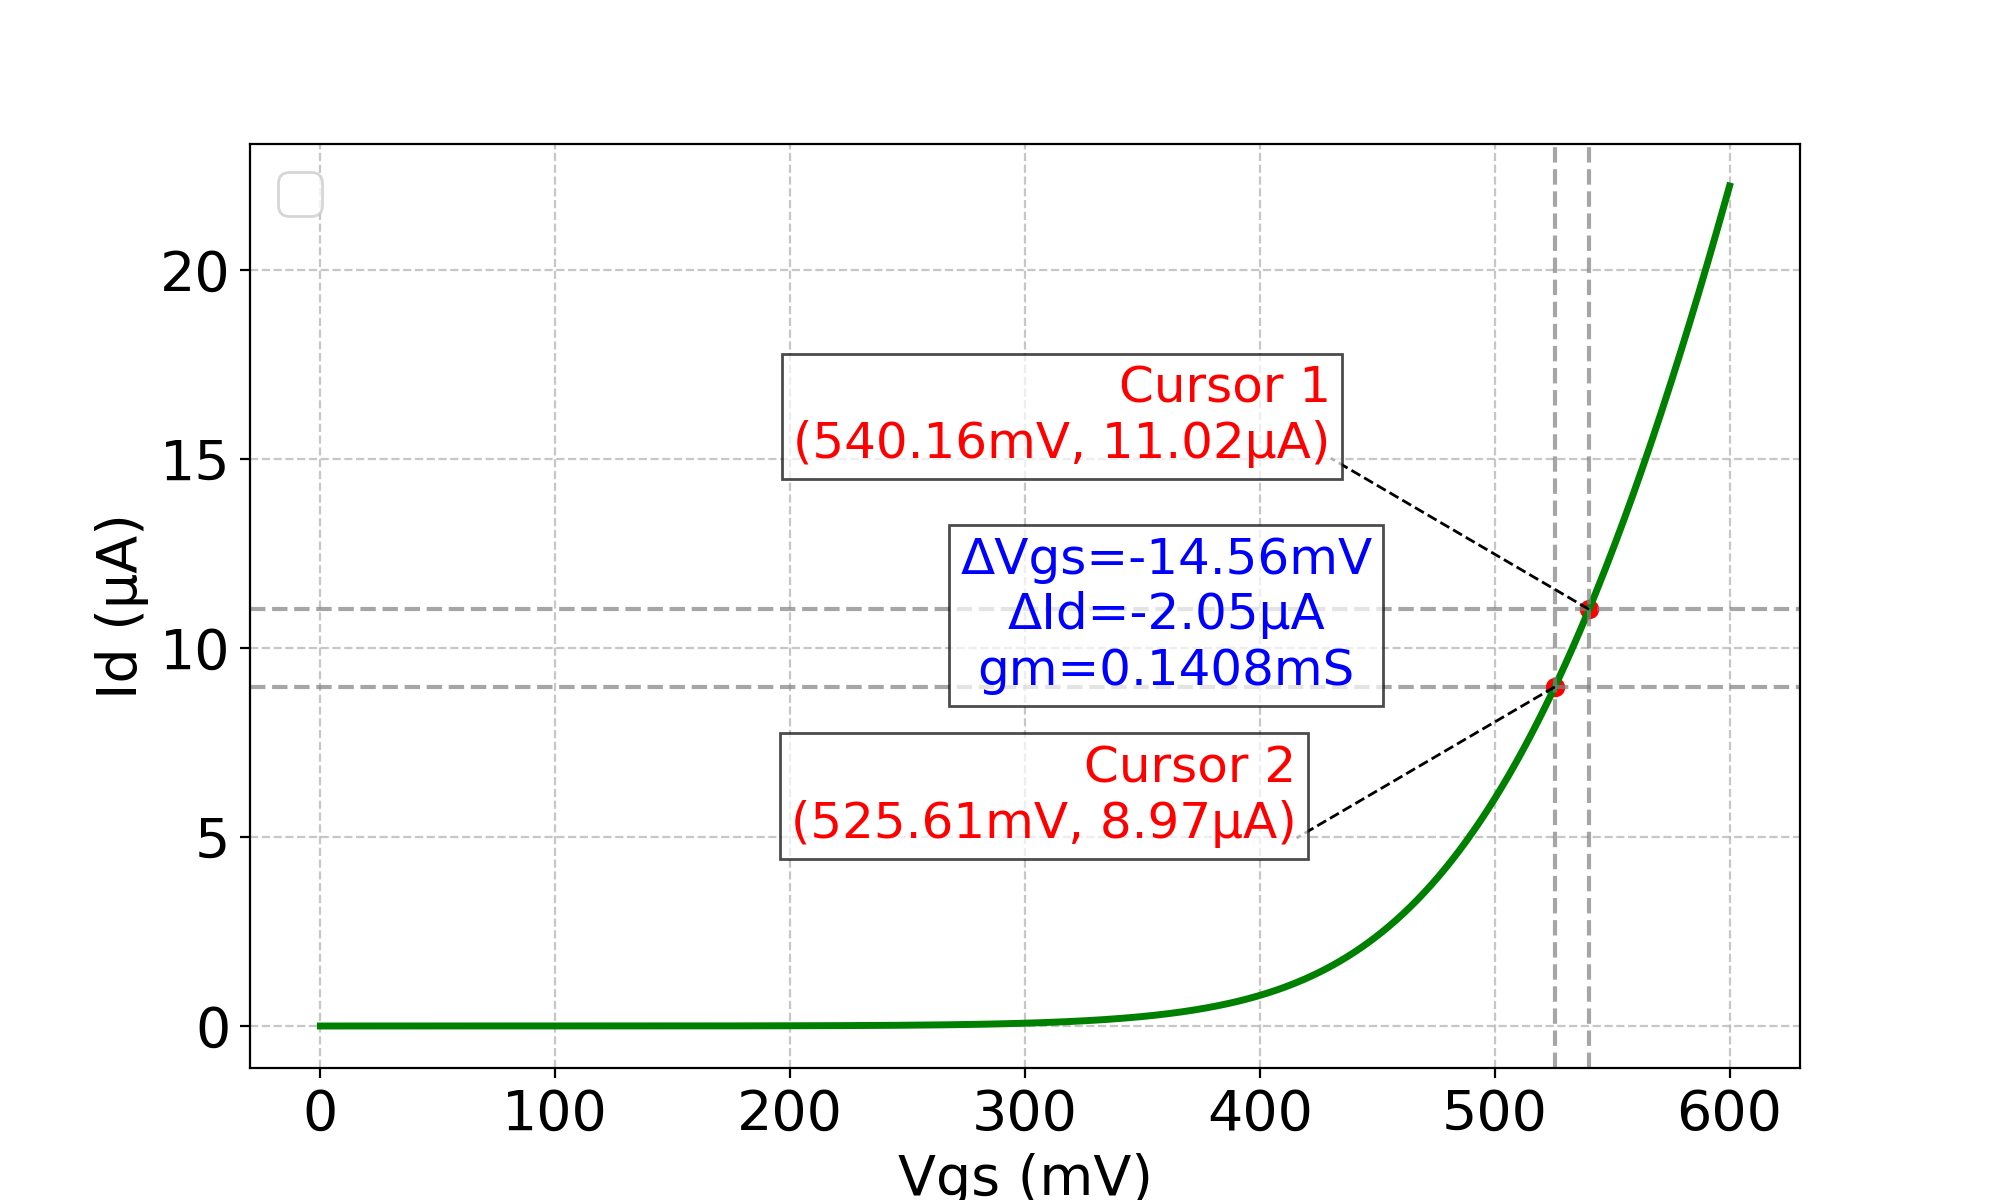
\includegraphics[height=0.25\textheight]{text/img/N-KP.png}
        \centering{(NMOS)}
    \end{minipage}
    \hfill
    \begin{minipage}{0.5\textwidth}
        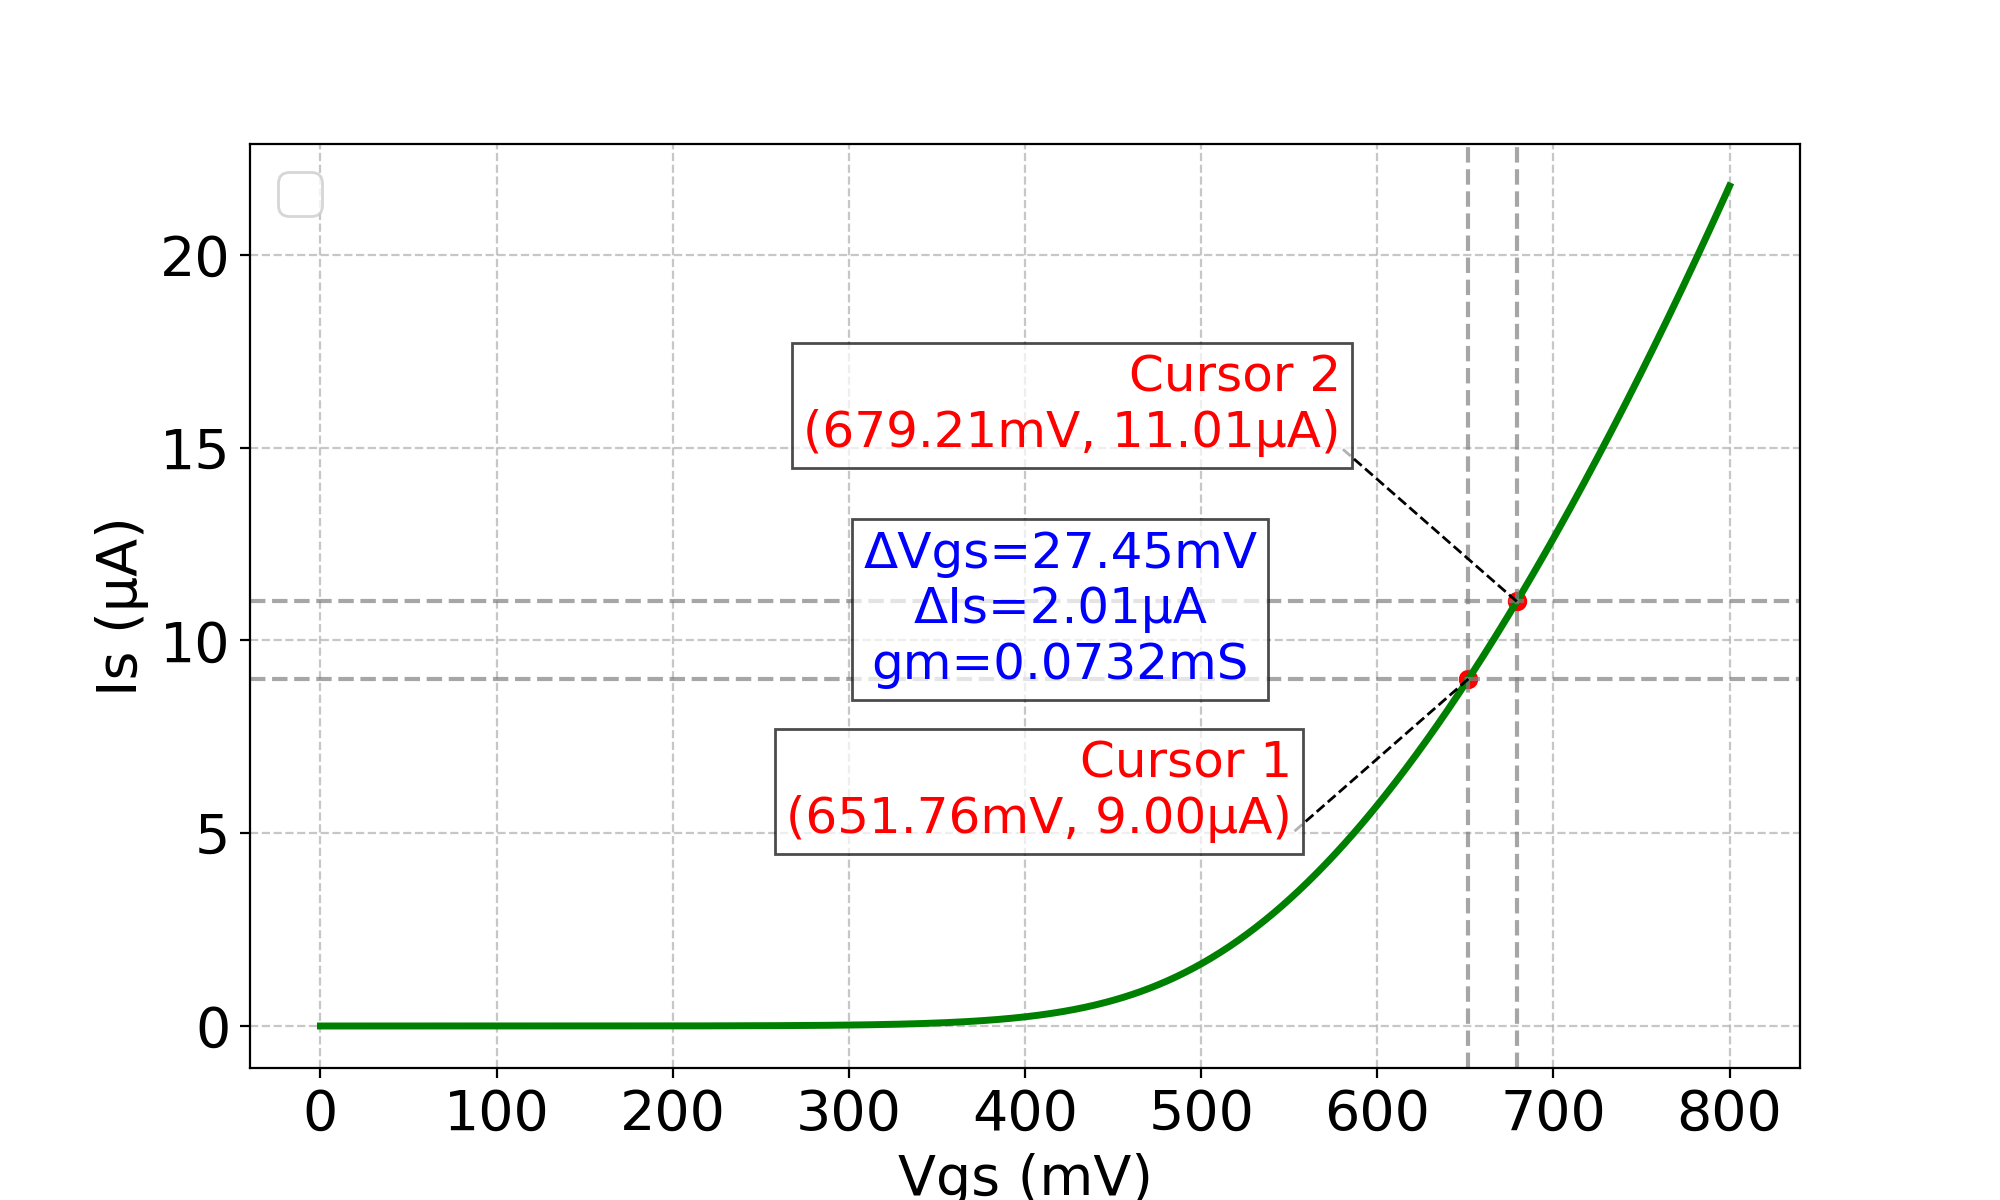
\includegraphics[height=0.25\textheight]{text/img/P-KP.png}
        \centering{(PMOS)}
    \end{minipage}
    \caption{\label{fig:graf_NP_KP} Závislost proudu tranzistorem NMOS i PMOS na napětí \(V_{GS}\)}
\end{figure}

Z uvedených kurzoru přímo vidímě strmost \(g_m\), \(140.8 \mu S\) pro NMOS a \(73.2 \mu S\) pro PMOS.
Mužeme tedy spočítat transkonduktanční parametr \(KP\) jako:\\


\Large
\(
    KP = \frac{g_m^2\cdot L}{2\cdot|I_D|\cdot W}
\)
\normalsize

Tedy pro NMOS:

\Large
\(
    KP_N = \frac{g_{m-N}^2\cdot L}{2\cdot|I_{D-N}|\cdot W} = \frac{(140.8\mu)^2\cdot1\mu}{2\cdot10\mu\cdot5\mu} = 198.2\mu A V^{-2} \cong 200 \mu A V^{-2}
\)
\normalsize

A PMOS:

\Large
\(
    KP_P = \frac{g_{m-P}^2\cdot L}{2\cdot|I_{D-P}|\cdot W} = \frac{(73.2\mu)^2\cdot1\mu}{2\cdot10\mu\cdot5\mu} = 53.6\mu A V^{-2} \cong  50 \mu A V^{-2}
\)
\normalsize
  \newpage
  \subsection{Prahové napětí \(U_{TH0}\)}  
    
\begin{figure}[H]
    Mezi uzly \(V_{CC}\) a \(GND\) je umístěn napěťový zdroj s napětím \(V_{CC} = 1.8 [V]\), pro zjednodušení jen není uveden ve schematu, což bude platit i u dalších zapojení.

    \vspace{8mm}
    \begin{minipage}{0.5\textwidth}
        \begin{circuitikz}[scale=1, transform shape] 
            \draw
              % MOSFET transistor with labels for drain (D), gate (G), source (S), and bulk (B)
              (0,0) node[nmos, bulk] (mos) {}
              (mos.drain) node[left] {M1}
            
              % Gate voltage source VGS
              (mos.gate) to[short, -] ++(-2,0) to[voltage source, l^=$V_{GS}$] ++(0,-1.5) node[ground] {}
              
              % Drain voltage source VDS (vertical)
              (mos.drain) to[short, -] ++(0,1) -- ++(2,0) -- ++(0,-1) to[voltage source, l^=$V_{DS} $] ++(0,-2) -- (2,-1.5) node[ground] {}
              
              % Source connected to ground, aligned with VGS ground
              (mos.source) to[short, -] (0,-1.5) node[ground] {}
              
              % Bulk (body) connection to ground
              (mos.bulk) to[short, -] (0.5, 0) -- ++(0,-1) -- ++(-0.5,0)  node[circle,fill,inner sep=1pt] (myNode) {}
            ;
        \end{circuitikz}

        \vspace{5mm}
        \centering{(NMOS)}
    \end{minipage}
    \hfill
    \begin{minipage}{0.5\textwidth}
        \begin{circuitikz}[scale=1, transform shape] 
            \draw
              % MOSFET transistor with labels for drain (D), gate (G), source (S), and bulk (B)
              (0,0) node[pmos, bulk] (mos) {}
              (mos.drain) node[left] {M1}
            
              % Gate voltage source VGS
              (mos.gate) to[short, -] (-2,0) to[voltage source, l^=$V_{GS}$] (-2,2) -- ++(2,0) node[circle,fill,inner sep=1pt] (myNode) {}
              
              % Drain voltage source VDS (vertical)
              (mos.source) to[short, -] (0,2) -- ++(2,0) -- ++(0,-1) to[voltage source, l^=$V_{DS} $] ++(0,-2) -- (2,-1.5) -- (0,-1.5) -- (mos.drain)
              
              % Source connected to ground, aligned with VGS ground
              %   (mos.source) to[short, -] (0,-1.5) node[ground] {}
              
              % Bulk (body) connection to ground
              (mos.bulk) to[short, -] (0.5, 0) -- ++(0,1) -- ++(-0.5,0)  node[circle,fill,inner sep=1pt] (myNode) {}

              (2,2)  to[short, *-o] ++(1,0) node[above, right]{$V_{CC}$}
            ;
        \end{circuitikz}

        \vspace{5mm} 
        \centering{(PMOS)}
    \end{minipage}
    \caption{\label{cod:cod_NP_WL_const} Zapojení pro určení \(U_{TH0}\) pro tranzistor NMOS a PMOS}
\end{figure}

\newpage
\subsubsection{Prahové napětí \(U_{TH0}\) při konstantním poměru \(W/L = 5\)}
\begin{lstlisting}[language=Spice, caption={Použitý kod simulace při konstantním poměru \(W/L = 5\)}]
.lib cmos018.txt
.STEP param lset list 0.18u, 0.3u, 0.5u, 0.8u, 1u, 2u, 3u, 5u, 10u
.param wset = 5*lset
.DC VGS 0.1 0.6 1m
.MEAS DC UTH FIND V(VG) WHEN Id(M1)=500n
\end{lstlisting}

\begin{figure}[H]
    \begin{minipage}{0.5\textwidth}
        \centering
        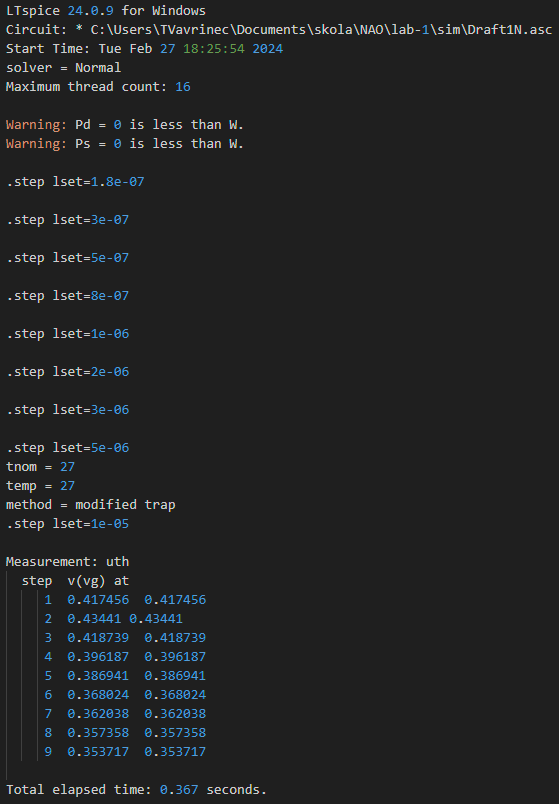
\includegraphics[height=0.4\textheight]{log/N-UTH0-WL_const.png}
        \centering{(NMOS)}
    \end{minipage}
    \hfill
    \begin{minipage}{0.5\textwidth}
        \centering
        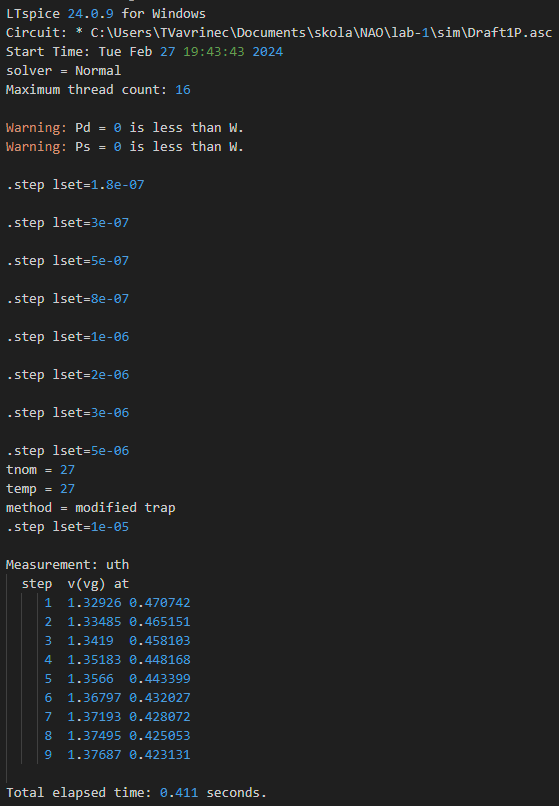
\includegraphics[height=0.4\textheight]{log/P-UTH0-WL_const.png}
        \centering{(PMOS)}
    \end{minipage}
    \caption{\label{fig:log_NP_WL_const} Printscreeny logů simulací při konstantním poměru \(W/L = 5\) pro NMOS i PMOS}
\end{figure}

\begin{table}[H]
    \begin{minipage}{0.5\textwidth}
        \centering
        \begin{tabular}{|c|c|}
            \hline
            \(L [\mu m]\) & \(U_{TH0} [V]\) \\ \hline
            0.18	      & 0.417456        \\ \hline
            0.3	          & 0.434410        \\ \hline
            0.5	          & 0.418739        \\ \hline
            0.8	          & 0.396187        \\ \hline
            1	          & 0.386941        \\ \hline
            2	          & 0.368024        \\ \hline
            3	          & 0.362038        \\ \hline
            5	          & 0.357358        \\ \hline
            10	          & 0.353717        \\ \hline
        \end{tabular}

        \vspace{5mm}
        \centering{(NMOS)}
    \end{minipage}
    \hfill
    \begin{minipage}{0.5\textwidth}
        \centering
        \begin{tabular}{|c|c|}
            \hline
            \(L [\mu m]\) & \(U_{TH0} [V]\) \\ \hline
            0.18          & 0.470742        \\ \hline
            0.3	          & 0.465151        \\ \hline
            0.5	          & 0.458103        \\ \hline
            0.8	          & 0.448168        \\ \hline
            1             & 0.443399        \\ \hline
            2  	          & 0.432027        \\ \hline
            3  	          & 0.428072        \\ \hline
            5  	          & 0.425053        \\ \hline
            10 	          & 0.423131        \\ \hline
        \end{tabular}

        \vspace{5mm}
        \centering{(PMOS)}
    \end{minipage}

    \caption{\label{tab:N_wl_const} Výsledky simulace při konstantním poměru \(W/L = 5\)}
\end{table}

\newpage
\subsubsection{Prahové napětí \(U_{TH0}\) při různém poměru \(W/L\)}
\begin{lstlisting}[language=Spice, caption={Použitý kod simulace při různém poměru \(W/L\)}]
.lib cmos018.txt
.param wset=table(n, 1,0.22u, 2,1u, 3,2u, 4,2u, 5,5u, 6,5u, 7,10u, 8,10u, 9,40u)
.param lset=table(n, 1,0.18u, 2,0.5u, 3,0.5u, 4,1u, 5,1u, 6,2u, 7,5u, 8,10u, 9,10u)
.step param n 1 9 1
.meas DC UTH FIND V(VG) WHEN Id(M1)=100n*wset/lset
.dc VGS2 0 1 1m
\end{lstlisting}

\begin{figure}[H]
    \begin{minipage}{0.5\textwidth}
        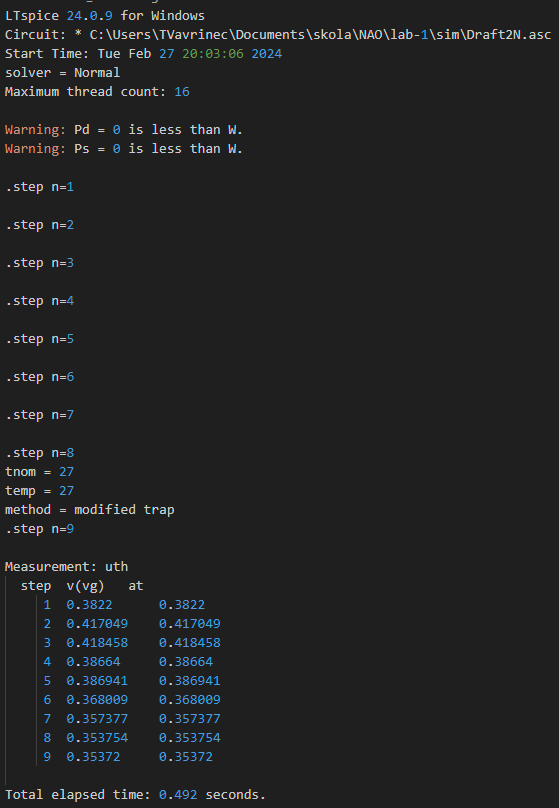
\includegraphics[height=0.4\textheight]{log/N-UTH00-WL_dinamic.png}
        \centering{(NMOS)}
    \end{minipage}
    \hfill
    \begin{minipage}{0.5\textwidth}
        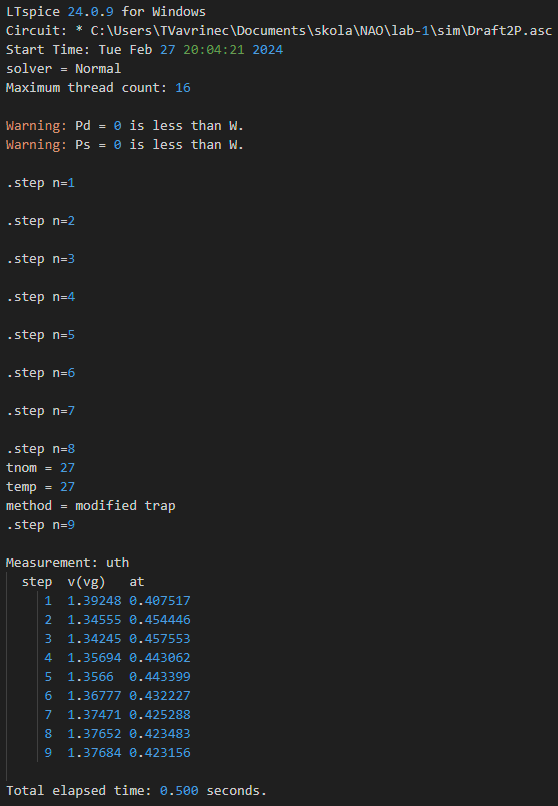
\includegraphics[height=0.4\textheight]{log/P-UTH00-WL_dinamic.png}
        \centering{(PMOS)}
    \end{minipage}
    \caption{\label{fig:log_NP_WL_const} Printscreeny logů simulací ruzných pomněru \(W/L\) pro NMOS i PMOS}
\end{figure}

\begin{table}[H]
    \begin{minipage}{0.5\textwidth}
        \centering
        \begin{tabular}{|c|c|c|}
            \hline
            \(L [\mu m]\) & \(W [\mu m]\) & \(U_{TH0} [V]\) \\ \hline
            0.22          & 0.18          & 0.382200        \\ \hline
            1	          & 0.5           & 0.417049	    \\ \hline
            2	          & 0.5           & 0.418458	    \\ \hline
            2	          & 1             & 0.386640        \\ \hline
            5             & 1             & 0.386941	    \\ \hline
            5  	          & 2             & 0.368009	    \\ \hline
            10 	          & 5             & 0.357377	    \\ \hline
            10 	          & 10            & 0.353754	    \\ \hline
            40 	          & 10            & 0.353720        \\ \hline
        \end{tabular}

        \vspace{5mm}
        \centering{(NMOS)}
    \end{minipage}
    \hfill
    \begin{minipage}{0.5\textwidth}
        \centering
        \begin{tabular}{|c|c|c|}
            \hline
            \(L [\mu m]\) & \(W [\mu m]\) & \(U_{TH0} [V]\) \\ \hline
            0.22          & 0.18          & 0.407517        \\ \hline
            1	          & 0.5           & 0.454446        \\ \hline
            2	          & 0.5           & 0.457553        \\ \hline
            2	          & 1             & 0.443062        \\ \hline
            5             & 1             & 0.443399        \\ \hline
            5  	          & 2             & 0.432227        \\ \hline
            10 	          & 5             & 0.425288        \\ \hline
            10 	          & 10            & 0.423483        \\ \hline
            40 	          & 10            & 0.423156        \\ \hline
        \end{tabular}

        \vspace{5mm}
        \centering{(PMOS)}
    \end{minipage}

    \caption{\label{tab:N_wl_const} Výsledky simulace při různém poměru \(W/L = 5\)}
\end{table}

  \newpage
  \subsection{Závislost prahového napětí \(U_{TH}\) na napětí bulku}  
    \begin{figure}[H]
    \begin{minipage}{0.5\textwidth}
        \begin{circuitikz}[scale=1, transform shape] 
            \draw
                % MOSFET transistor with labels for drain (D), gate (G), source (S), and bulk (B)
                (0,0) node[nmos, bulk] (mos) {}
                (mos.drain) node[left] {M1}
                
                % Gate voltage source VGS
                (mos.gate) to[short, -] ++(-2,0) -- ++(0,0) to[voltage source, l^=$V_{GS}$] ++(0,-1.5) -- ++(2.99,0) node[circle,fill,inner sep=1pt] (myNode) {}
                
                % Drain voltage source VDS (vertical)
                (mos.drain) to[short, -] ++(0,1) -- ++(2,0) -- ++(0,-0.5) to[voltage source, l^=$V_{DS} $] ++(0,-2) -- ++(0,-0.78) -- ++(-2,0) {}
                
                % Source connected to ground, aligned with VGS ground
                (mos.source) to[short, -] (0,-2.3) to[voltage source, l_=$V_{BS} $] (0,-2) -- (0, -3) node[ground] {}
                
                % Bulk (body) connection to ground
                (mos.bulk) to[short, -] (1, 0) -- ++(0,-0.5)  node[ground] {}
            ;
        \end{circuitikz}

        \vspace{5mm}
        \centering{(NMOS)}
    \end{minipage}
    \hfill
    \begin{minipage}{0.5\textwidth}
        \begin{circuitikz}[scale=1, transform shape] 
            \draw
                % MOSFET transistor with labels for drain (D), gate (G), source (S), and bulk (B)
                (0,-1) node[pmos, bulk] (mos) {}
                (mos.drain) node[left] {M1}
                
                % Gate voltage source VGS
                (mos.gate) to[short, -] (-2,-1) to[voltage source, l^=$V_{GS}$] (-2,0) -- ++(2,0) node[circle,fill,inner sep=1pt] (myNode) {}

                (0,0) -- ++(2,0) to[voltage source, l^=$V_{DS} $] ++(0,-1.5) -- ++(0,-0.5) -- (1,-2) -* (0,-2) node[circle,fill,inner sep=1pt] (myNode) {}


                % Drain voltage source VDS (vertical)
                (mos.source) to[short, -] (0,0.5) to[voltage source, l^=$V_{SB} $] (0,1.5) -- (0,2) -- ++(1,0) -- ++(0,-3) -- (1,-1) -- (mos.bulk) {}
                %   (mos.source) to[short, -] (0,2) -- ++(2,0) -- ++(0,-1) to[voltage source, l^=$V_{DS} $] ++(0,-2) -- (2,-1.5) -- (0,-1.5) -- (mos.drain)
                
                % Source connected to ground, aligned with VGS ground
                (mos.drain) to[short, -] (0,-2.6) node[ground] {}

                %   (2,2)  to[short, *-o] ++(1,0) node[above, right]{$V_{CC}$}
            ;
        \end{circuitikz}

        \vspace{5mm} 
        \centering{(PMOS)}
    \end{minipage}
    \caption{\label{cod:cod_NP_WL_const} Zapojení pro určení závislosti \(U_{TH}\) na napětí bulku pro tranzistor NMOS a PMOS}
\end{figure}

\begin{lstlisting}[language=Spice, caption={Kod simulace pro určení závislosti \(U_{TH}\) na napětí bulku, pro NMOS}]
    .lib modely/cmos018.txt
    .STEP VSB 0 1 10m
    .DC VGS 0 1 1m
    .MEAS DC UTH FIND 'V(VG)-V(SB)' WHEN Id(M1)=500n    ; Pro NMOS
    .MEAS DC UTH FIND '1.8-V(VG)' WHEN Is(M1)=500n      ; Pro PMOS
\end{lstlisting}


\begin{figure}[h]
    \centering
    \includegraphics[height=0.3\textheight]{text/img/NP-bulkEfekt.png}
    \caption{\label{fig:graf_NP_KP} Závislost proudu tranzistorem NMOS i PMOS na napětí \(V_{GS}\)}
\end{figure}

Z grafu je patrné, že \(U_{TH}\) je na napětí \(U_{SB}\) závislé zhruba lineárně.

\begin{figure}[H]
    \begin{minipage}{0.5\textwidth}
        \begin{circuitikz}[scale=1, transform shape] 
            \draw
                % MOSFET transistor with labels for drain (D), gate (G), source (S), and bulk (B)
                (0,0) node[nmos, bulk] (mos) {}
                (mos.drain) node[left] {M1}
                
                % Gate voltage source VGS
                (mos.gate) to[short, -] ++(-2,0) -- ++(0,0) to[voltage source, l^=$V_{GS}$] ++(0,-1.5) -- ++(2.99,0) node[circle,fill,inner sep=1pt] (myNode) {}
                
                % Drain voltage source VDS (vertical)
                (mos.drain) to[short, -] ++(0,1) -- ++(2,0) -- ++(0,-0.5) to[voltage source, l^=$V_{DS} $] ++(0,-2) -- ++(0,-0.78) -- ++(-2,0) {}
                
                % Source connected to ground, aligned with VGS ground
                (mos.source) to[short, -] (0,-2.3) to[voltage source, l_=$V_{BS} $] (0,-2) -- (0, -3) node[ground] {}
                
                % Bulk (body) connection to ground
                (mos.bulk) to[short, -] (1, 0) -- ++(0,-0.5)  node[ground] {}
            ;
        \end{circuitikz}

        \vspace{5mm}
        \centering{(NMOS)}
    \end{minipage}
    \hfill
    \begin{minipage}{0.5\textwidth}
        \begin{circuitikz}[scale=1, transform shape] 
            \draw
                % MOSFET transistor with labels for drain (D), gate (G), source (S), and bulk (B)
                (0,-1) node[pmos, bulk] (mos) {}
                (mos.drain) node[left] {M1}
                
                % Gate voltage source VGS
                (mos.gate) to[short, -] (-2,-1) to[voltage source, l^=$V_{GS}$] (-2,0) -- ++(2,0) node[circle,fill,inner sep=1pt] (myNode) {}

                (0,0) -- ++(2,0) to[voltage source, l^=$V_{DS} $] ++(0,-1.5) -- ++(0,-0.5) -- (1,-2) -* (0,-2) node[circle,fill,inner sep=1pt] (myNode) {}


                % Drain voltage source VDS (vertical)
                (mos.source) to[short, -] (0,0.5) to[voltage source, l^=$V_{SB} $] (0,1.5) -- (0,2) -- ++(1,0) -- ++(0,-3) -- (1,-1) -- (mos.bulk) {}
                %   (mos.source) to[short, -] (0,2) -- ++(2,0) -- ++(0,-1) to[voltage source, l^=$V_{DS} $] ++(0,-2) -- (2,-1.5) -- (0,-1.5) -- (mos.drain)
                
                % Source connected to ground, aligned with VGS ground
                (mos.drain) to[short, -] (0,-2.6) node[ground] {}

                %   (2,2)  to[short, *-o] ++(1,0) node[above, right]{$V_{CC}$}
            ;
        \end{circuitikz}

        \vspace{5mm} 
        \centering{(PMOS)}
    \end{minipage}
    \caption{\label{cod:cod_NP_WL_const} Zapojení pro určení závislosti \(U_{TH}\) na napětí bulku pro tranzistor NMOS a PMOS}
\end{figure}

\begin{lstlisting}[language=Spice, caption={Kod simulace pro určení závislosti \(U_{TH}\) na napětí bulku, pro NMOS}]
    .lib modely/cmos018.txt
    .STEP VSB 0 1 10m
    .DC VGS 0 1 1m
    .MEAS DC UTH FIND 'V(VG)-V(SB)' WHEN Id(M1)=500n    ; Pro NMOS
    .MEAS DC UTH FIND '1.8-V(VG)' WHEN Is(M1)=500n      ; Pro PMOS
\end{lstlisting}


\begin{figure}[h]
    \centering
    \includegraphics[height=0.3\textheight]{text/img/NP-bulkEfekt.png}
    \caption{\label{fig:graf_NP_KP} Závislost proudu tranzistorem NMOS i PMOS na napětí \(V_{GS}\)}
\end{figure}

Z grafu je patrné, že \(U_{TH}\) je na napětí \(U_{SB}\) závislé zhruba lineárně.

\begin{figure}[H]
    \begin{minipage}{0.5\textwidth}
        \begin{circuitikz}[scale=1, transform shape] 
            \draw
                % MOSFET transistor with labels for drain (D), gate (G), source (S), and bulk (B)
                (0,0) node[nmos, bulk] (mos) {}
                (mos.drain) node[left] {M1}
                
                % Gate voltage source VGS
                (mos.gate) to[short, -] ++(-2,0) -- ++(0,0) to[voltage source, l^=$V_{GS}$] ++(0,-1.5) -- ++(2.99,0) node[circle,fill,inner sep=1pt] (myNode) {}
                
                % Drain voltage source VDS (vertical)
                (mos.drain) to[short, -] ++(0,1) -- ++(2,0) -- ++(0,-0.5) to[voltage source, l^=$V_{DS} $] ++(0,-2) -- ++(0,-0.78) -- ++(-2,0) {}
                
                % Source connected to ground, aligned with VGS ground
                (mos.source) to[short, -] (0,-2.3) to[voltage source, l_=$V_{BS} $] (0,-2) -- (0, -3) node[ground] {}
                
                % Bulk (body) connection to ground
                (mos.bulk) to[short, -] (1, 0) -- ++(0,-0.5)  node[ground] {}
            ;
        \end{circuitikz}

        \vspace{5mm}
        \centering{(NMOS)}
    \end{minipage}
    \hfill
    \begin{minipage}{0.5\textwidth}
        \begin{circuitikz}[scale=1, transform shape] 
            \draw
                % MOSFET transistor with labels for drain (D), gate (G), source (S), and bulk (B)
                (0,-1) node[pmos, bulk] (mos) {}
                (mos.drain) node[left] {M1}
                
                % Gate voltage source VGS
                (mos.gate) to[short, -] (-2,-1) to[voltage source, l^=$V_{GS}$] (-2,0) -- ++(2,0) node[circle,fill,inner sep=1pt] (myNode) {}

                (0,0) -- ++(2,0) to[voltage source, l^=$V_{DS} $] ++(0,-1.5) -- ++(0,-0.5) -- (1,-2) -* (0,-2) node[circle,fill,inner sep=1pt] (myNode) {}


                % Drain voltage source VDS (vertical)
                (mos.source) to[short, -] (0,0.5) to[voltage source, l^=$V_{SB} $] (0,1.5) -- (0,2) -- ++(1,0) -- ++(0,-3) -- (1,-1) -- (mos.bulk) {}
                %   (mos.source) to[short, -] (0,2) -- ++(2,0) -- ++(0,-1) to[voltage source, l^=$V_{DS} $] ++(0,-2) -- (2,-1.5) -- (0,-1.5) -- (mos.drain)
                
                % Source connected to ground, aligned with VGS ground
                (mos.drain) to[short, -] (0,-2.6) node[ground] {}

                %   (2,2)  to[short, *-o] ++(1,0) node[above, right]{$V_{CC}$}
            ;
        \end{circuitikz}

        \vspace{5mm} 
        \centering{(PMOS)}
    \end{minipage}
    \caption{\label{cod:cod_NP_WL_const} Zapojení pro určení závislosti \(U_{TH}\) na napětí bulku pro tranzistor NMOS a PMOS}
\end{figure}

\begin{lstlisting}[language=Spice, caption={Kod simulace pro určení závislosti \(U_{TH}\) na napětí bulku, pro NMOS}]
    .lib modely/cmos018.txt
    .STEP VSB 0 1 10m
    .DC VGS 0 1 1m
    .MEAS DC UTH FIND 'V(VG)-V(SB)' WHEN Id(M1)=500n    ; Pro NMOS
    .MEAS DC UTH FIND '1.8-V(VG)' WHEN Is(M1)=500n      ; Pro PMOS
\end{lstlisting}


\begin{figure}[h]
    \centering
    \includegraphics[height=0.3\textheight]{text/img/NP-bulkEfekt.png}
    \caption{\label{fig:graf_NP_KP} Závislost proudu tranzistorem NMOS i PMOS na napětí \(V_{GS}\)}
\end{figure}

Z grafu je patrné, že \(U_{TH}\) je na napětí \(U_{SB}\) závislé zhruba lineárně.

\input{text/table/bulkEfekt.tex}



  \newpage
  \subsection{Závislost modulace délky kanálu (\(\lambda\)) na délce kanálu (\(L\))}
    \begin{figure}[H]
    \vspace{8mm}
    \begin{minipage}{0.5\textwidth}
        \begin{circuitikz}[scale=1, transform shape] 
            \draw
              % MOSFET transistor with labels for drain (D), gate (G), source (S), and bulk (B)
              (0,0) node[nmos, bulk] (mos) {}
              (mos.drain) node[left] {M1}
            
              % Gate voltage source VGS
              (mos.gate) to[short, -] ++(-2,0) to[voltage source, l^=$V_{GS}$] ++(0,-1.5) node[ground] {}
              
              % Drain voltage source VDS (vertical)
              (mos.drain) to[short, -] ++(0,1) -- ++(2,0) -- ++(0,-1) to[voltage source, l^=$V_{DS} $] ++(0,-2) -- (2,-1.5) node[ground] {}
              
              % Source connected to ground, aligned with VGS ground
              (mos.source) to[short, -] (0,-1.5) node[ground] {}
              
              % Bulk (body) connection to ground
              (mos.bulk) to[short, -] (0.5, 0) -- ++(0,-1) -- ++(-0.5,0)  node[circle,fill,inner sep=1pt] (myNode) {}
            ;
        \end{circuitikz}

        \vspace{5mm}
        \centering{(NMOS)}
    \end{minipage}
    \hfill
    \begin{minipage}{0.5\textwidth}
        \begin{circuitikz}[scale=1, transform shape] 
            \draw
              % MOSFET transistor with labels for drain (D), gate (G), source (S), and bulk (B)
              (0,0) node[pmos, bulk] (mos) {}
              (mos.drain) node[left] {M1}
                          
              % Gate voltage source VGS
              (mos.gate) to[short, -] (-2,0) to[voltage source, l^=$V_{GS}$] (-2,2) -- ++(2,0) node[circle,fill,inner sep=1pt] (myNode) {}
              
              % Drain voltage source VDS (vertical)
              (mos.source) to[short, -] (0,2) -- ++(2,0) -- ++(0,-1) to[voltage source, l^=$V_{DS} $] ++(0,-2) -- (2,-1.5) -- (0,-1.5)
              
              % Source connected to ground, aligned with VGS ground
              (mos.drain) to[short, ] (0,-1.5) node[circle,fill,inner sep=1pt] (myNode) {} (0,-1.5) node[ground] {}

              % Bulk (body) connection to ground
              (mos.bulk) to[short, -] (0.5, 0) -- ++(0,1) -- ++(-0.5,0)  node[circle,fill,inner sep=1pt] (myNode) {}

            %   (2,2)  to[short, *-o] ++(1,0) node[above, right]{$V_{CC}$}
            ;
        \end{circuitikz}

        \vspace{5mm} 
        \centering{(PMOS)}
    \end{minipage}
    \caption{\label{cod:cod_NP_WL_const} Zapojení pro určení závislosti modulace delky kanálu \(\lambda\) na delce kanálu \(L\)}
\end{figure}

\begin{lstlisting}[language=Spice, caption={ \centering Kod simulace použítí pro získání závislosti \\ modulované délky kanálu \(\lambda\) na délce kanálu \(L\)}, label={cod:cod_lambda}]
.lib cmos018.txt
.step param lset 0.1u 10u 0.02u
.param wset=5*lset
.meas DC ID1 FIND Id(M1) WHEN V(VD)=0.5
.meas DC ID2 FIND Id(M1) WHEN V(VD)=1.3
.meas DC ID0 FIND Id(M1) WHEN V(VD)=0.9
.meas rout param (1.3-0.5)/(ID2-ID1)
.meas lambda param 1/(ID0*rout)
.dc UDS 0.5 1.3 10m
\end{lstlisting}

\vspace{-7mm}
\begin{figure}[h]
    \centering
    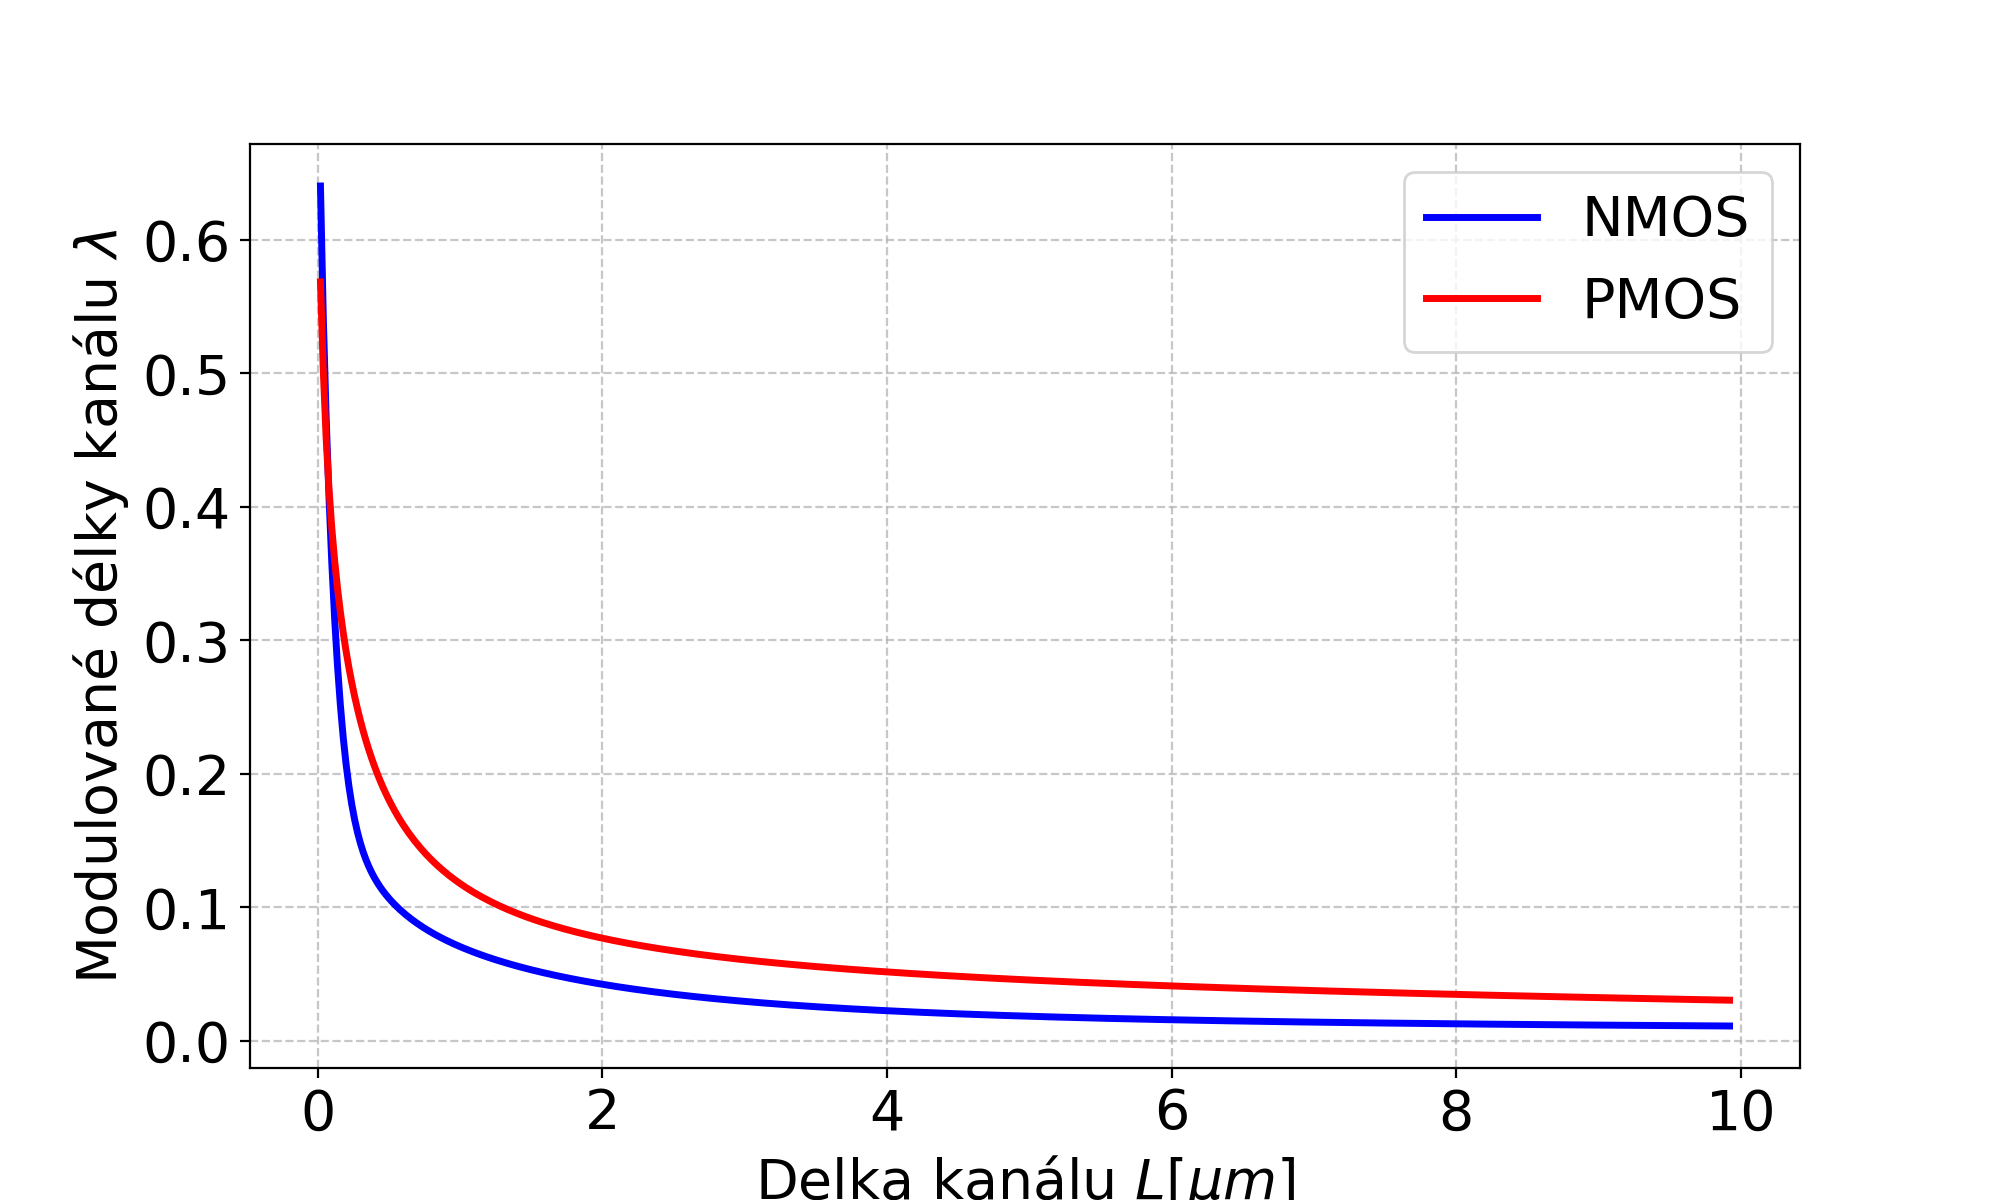
\includegraphics[height=0.28\textheight]{text/img/lambda.png}
    \caption{\label{fig:lambda} Závislost parametru \(\lambda\) na délce kanálu \(L\) při poměru \(W/L = 5\)}
\end{figure}

\vspace{-1mm}
\begin{figure}[H]
    \vspace{8mm}
    \begin{minipage}{0.5\textwidth}
        \begin{circuitikz}[scale=1, transform shape] 
            \draw
              % MOSFET transistor with labels for drain (D), gate (G), source (S), and bulk (B)
              (0,0) node[nmos, bulk] (mos) {}
              (mos.drain) node[left] {M1}
            
              % Gate voltage source VGS
              (mos.gate) to[short, -] ++(-2,0) to[voltage source, l^=$V_{GS}$] ++(0,-1.5) node[ground] {}
              
              % Drain voltage source VDS (vertical)
              (mos.drain) to[short, -] ++(0,1) -- ++(2,0) -- ++(0,-1) to[voltage source, l^=$V_{DS} $] ++(0,-2) -- (2,-1.5) node[ground] {}
              
              % Source connected to ground, aligned with VGS ground
              (mos.source) to[short, -] (0,-1.5) node[ground] {}
              
              % Bulk (body) connection to ground
              (mos.bulk) to[short, -] (0.5, 0) -- ++(0,-1) -- ++(-0.5,0)  node[circle,fill,inner sep=1pt] (myNode) {}
            ;
        \end{circuitikz}

        \vspace{5mm}
        \centering{(NMOS)}
    \end{minipage}
    \hfill
    \begin{minipage}{0.5\textwidth}
        \begin{circuitikz}[scale=1, transform shape] 
            \draw
              % MOSFET transistor with labels for drain (D), gate (G), source (S), and bulk (B)
              (0,0) node[pmos, bulk] (mos) {}
              (mos.drain) node[left] {M1}
                          
              % Gate voltage source VGS
              (mos.gate) to[short, -] (-2,0) to[voltage source, l^=$V_{GS}$] (-2,2) -- ++(2,0) node[circle,fill,inner sep=1pt] (myNode) {}
              
              % Drain voltage source VDS (vertical)
              (mos.source) to[short, -] (0,2) -- ++(2,0) -- ++(0,-1) to[voltage source, l^=$V_{DS} $] ++(0,-2) -- (2,-1.5) -- (0,-1.5)
              
              % Source connected to ground, aligned with VGS ground
              (mos.drain) to[short, ] (0,-1.5) node[circle,fill,inner sep=1pt] (myNode) {} (0,-1.5) node[ground] {}

              % Bulk (body) connection to ground
              (mos.bulk) to[short, -] (0.5, 0) -- ++(0,1) -- ++(-0.5,0)  node[circle,fill,inner sep=1pt] (myNode) {}

            %   (2,2)  to[short, *-o] ++(1,0) node[above, right]{$V_{CC}$}
            ;
        \end{circuitikz}

        \vspace{5mm} 
        \centering{(PMOS)}
    \end{minipage}
    \caption{\label{cod:cod_NP_WL_const} Zapojení pro určení závislosti modulace delky kanálu \(\lambda\) na delce kanálu \(L\)}
\end{figure}

\begin{lstlisting}[language=Spice, caption={ \centering Kod simulace použítí pro získání závislosti \\ modulované délky kanálu \(\lambda\) na délce kanálu \(L\)}, label={cod:cod_lambda}]
.lib cmos018.txt
.step param lset 0.1u 10u 0.02u
.param wset=5*lset
.meas DC ID1 FIND Id(M1) WHEN V(VD)=0.5
.meas DC ID2 FIND Id(M1) WHEN V(VD)=1.3
.meas DC ID0 FIND Id(M1) WHEN V(VD)=0.9
.meas rout param (1.3-0.5)/(ID2-ID1)
.meas lambda param 1/(ID0*rout)
.dc UDS 0.5 1.3 10m
\end{lstlisting}

\vspace{-7mm}
\begin{figure}[h]
    \centering
    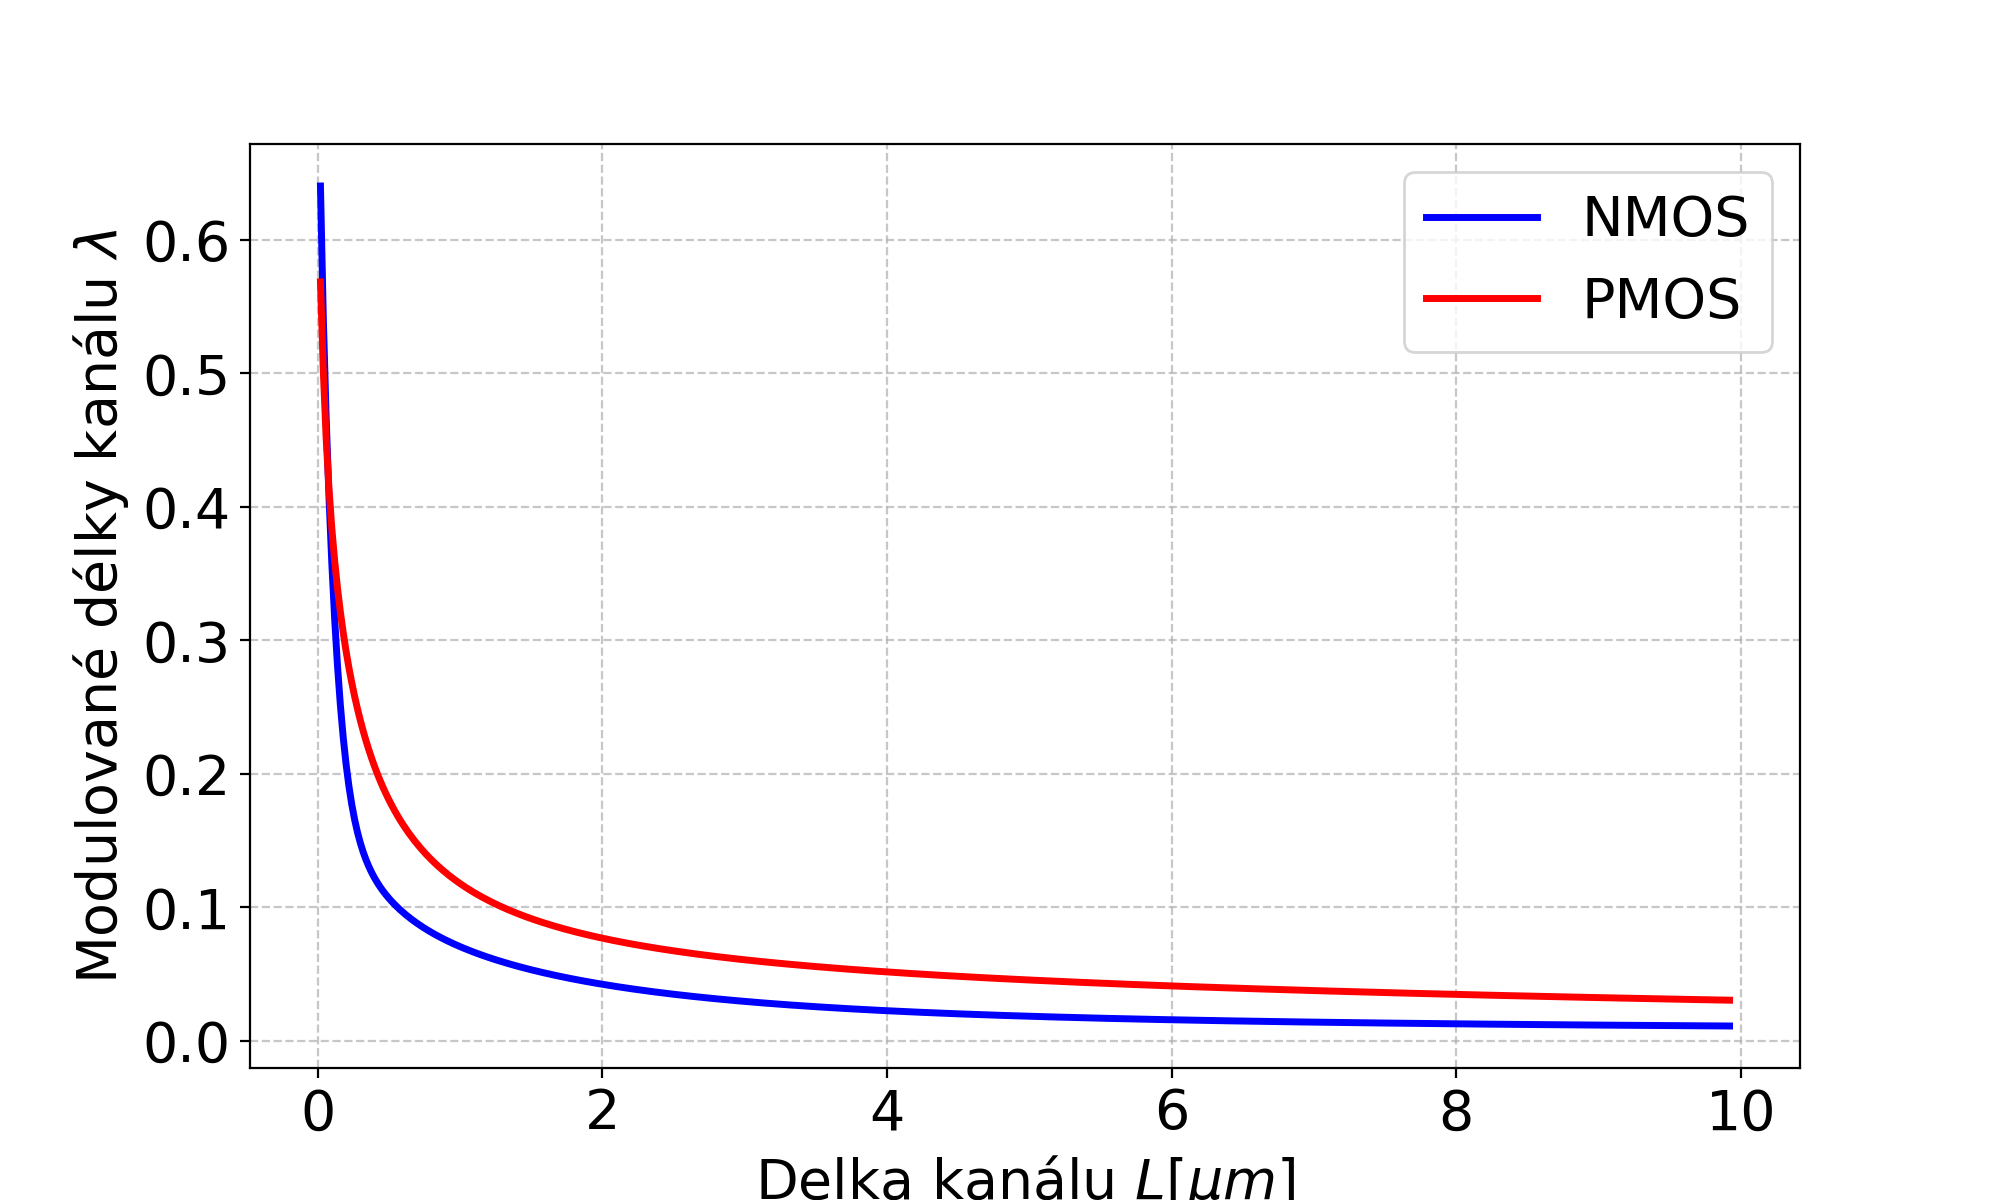
\includegraphics[height=0.28\textheight]{text/img/lambda.png}
    \caption{\label{fig:lambda} Závislost parametru \(\lambda\) na délce kanálu \(L\) při poměru \(W/L = 5\)}
\end{figure}

\vspace{-1mm}
\begin{figure}[H]
    \vspace{8mm}
    \begin{minipage}{0.5\textwidth}
        \begin{circuitikz}[scale=1, transform shape] 
            \draw
              % MOSFET transistor with labels for drain (D), gate (G), source (S), and bulk (B)
              (0,0) node[nmos, bulk] (mos) {}
              (mos.drain) node[left] {M1}
            
              % Gate voltage source VGS
              (mos.gate) to[short, -] ++(-2,0) to[voltage source, l^=$V_{GS}$] ++(0,-1.5) node[ground] {}
              
              % Drain voltage source VDS (vertical)
              (mos.drain) to[short, -] ++(0,1) -- ++(2,0) -- ++(0,-1) to[voltage source, l^=$V_{DS} $] ++(0,-2) -- (2,-1.5) node[ground] {}
              
              % Source connected to ground, aligned with VGS ground
              (mos.source) to[short, -] (0,-1.5) node[ground] {}
              
              % Bulk (body) connection to ground
              (mos.bulk) to[short, -] (0.5, 0) -- ++(0,-1) -- ++(-0.5,0)  node[circle,fill,inner sep=1pt] (myNode) {}
            ;
        \end{circuitikz}

        \vspace{5mm}
        \centering{(NMOS)}
    \end{minipage}
    \hfill
    \begin{minipage}{0.5\textwidth}
        \begin{circuitikz}[scale=1, transform shape] 
            \draw
              % MOSFET transistor with labels for drain (D), gate (G), source (S), and bulk (B)
              (0,0) node[pmos, bulk] (mos) {}
              (mos.drain) node[left] {M1}
                          
              % Gate voltage source VGS
              (mos.gate) to[short, -] (-2,0) to[voltage source, l^=$V_{GS}$] (-2,2) -- ++(2,0) node[circle,fill,inner sep=1pt] (myNode) {}
              
              % Drain voltage source VDS (vertical)
              (mos.source) to[short, -] (0,2) -- ++(2,0) -- ++(0,-1) to[voltage source, l^=$V_{DS} $] ++(0,-2) -- (2,-1.5) -- (0,-1.5)
              
              % Source connected to ground, aligned with VGS ground
              (mos.drain) to[short, ] (0,-1.5) node[circle,fill,inner sep=1pt] (myNode) {} (0,-1.5) node[ground] {}

              % Bulk (body) connection to ground
              (mos.bulk) to[short, -] (0.5, 0) -- ++(0,1) -- ++(-0.5,0)  node[circle,fill,inner sep=1pt] (myNode) {}

            %   (2,2)  to[short, *-o] ++(1,0) node[above, right]{$V_{CC}$}
            ;
        \end{circuitikz}

        \vspace{5mm} 
        \centering{(PMOS)}
    \end{minipage}
    \caption{\label{cod:cod_NP_WL_const} Zapojení pro určení závislosti modulace delky kanálu \(\lambda\) na delce kanálu \(L\)}
\end{figure}

\begin{lstlisting}[language=Spice, caption={ \centering Kod simulace použítí pro získání závislosti \\ modulované délky kanálu \(\lambda\) na délce kanálu \(L\)}, label={cod:cod_lambda}]
.lib cmos018.txt
.step param lset 0.1u 10u 0.02u
.param wset=5*lset
.meas DC ID1 FIND Id(M1) WHEN V(VD)=0.5
.meas DC ID2 FIND Id(M1) WHEN V(VD)=1.3
.meas DC ID0 FIND Id(M1) WHEN V(VD)=0.9
.meas rout param (1.3-0.5)/(ID2-ID1)
.meas lambda param 1/(ID0*rout)
.dc UDS 0.5 1.3 10m
\end{lstlisting}

\vspace{-7mm}
\begin{figure}[h]
    \centering
    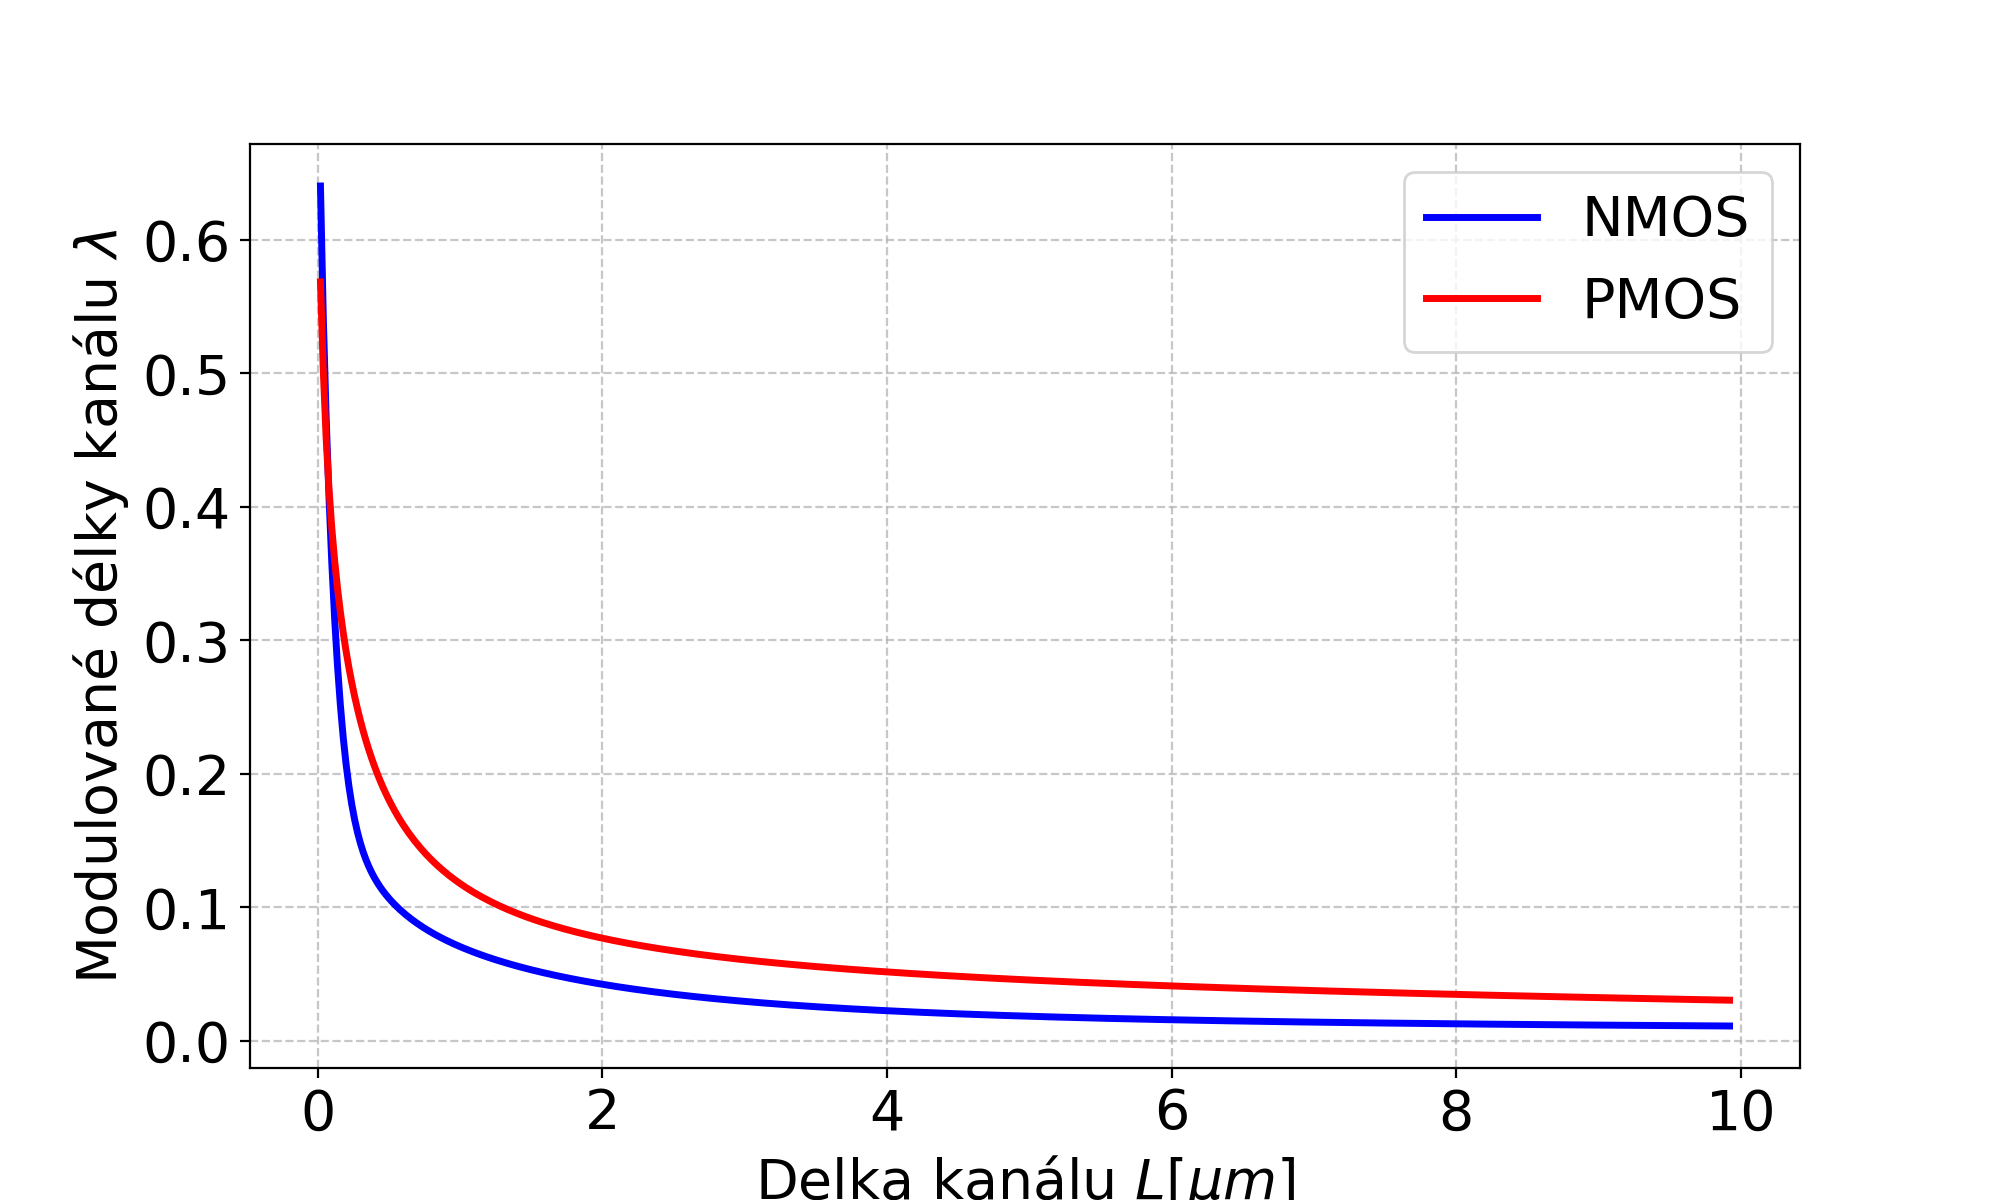
\includegraphics[height=0.28\textheight]{text/img/lambda.png}
    \caption{\label{fig:lambda} Závislost parametru \(\lambda\) na délce kanálu \(L\) při poměru \(W/L = 5\)}
\end{figure}

\vspace{-1mm}
\input{text/table/lambda.tex}




\section{Závěr}
  Porovnání obou verzí zesilovače.

\begin{table}[h]
    \centering
    \begin{tabular}{|l|c|c|c|}
        \hline
        \textbf{Typ zátěže} & \textbf{Zesílení \(A_{U0} [-]\)} & \textbf{Rychlost přeběhu  \(SR_{fell} [V/\mu s]\)} & \textbf{šířka pásma \(GBW [MHz]\)} \\ \hline
        Odporová            & 19                               & 3.5                                                & 8.43                               \\ \hline
        Aktivní             & 38                               & 5.0                                                & 8.12                               \\ \hline
    \end{tabular}
    \caption{Porovnání obou typů zátěže}
    \label{tab:zrcadla}
\end{table}

% \clearpage
% \section*{Reference}
% \printbibliography[heading=none]

\end{document}